\documentclass[12]{report}

%import packages for theoretical computer science stuff
\usepackage{amsmath}
\usepackage{amssymb}
\usepackage{amsthm}
\usepackage{mathrsfs}

%import packages for images
\usepackage{graphicx}
\usepackage{float}

%import packages for algorithms
\usepackage{algorithm}
\usepackage{algorithmic}
\usepackage{listings}
\usepackage{graphicx}

\usepackage{subfigure}
\usepackage{subcaption}
\usepackage{caption}
\usepackage{longtable}


%import packages for automata
\usepackage{tikz}
\usetikzlibrary{automata,positioning}
\usetikzlibrary{graphs,positioning}
\usetikzlibrary{chains,fit,shapes}

%setup document margins and spacing
\usepackage[margin=1in]{geometry}
\usepackage{setspace}
\onehalfspacing


%import packages for hyperlinks
\usepackage{hyperref}
\hypersetup{
    colorlinks=true,
    linkcolor=purple,
    filecolor=magenta,
    urlcolor=cyan,
}


%begin document
\begin{document}

\title{Machine Learning - House Prices Analysis}
%insert 5 members of the group
\author{Daniele Avolio : 242423\\
    \and
    Alessandro Fazio : 242422\\
    \and
    Merem Hassem Indiris\\
    \and
    Michele Vitale\\
    \and
    Lorenzo Piro\\}
\date{A.Y. 2022/2023}
\maketitle


\begin{titlepage}
    %insert a fullpage cover image without considering margins
    \noindent\makebox[\textwidth]{%
        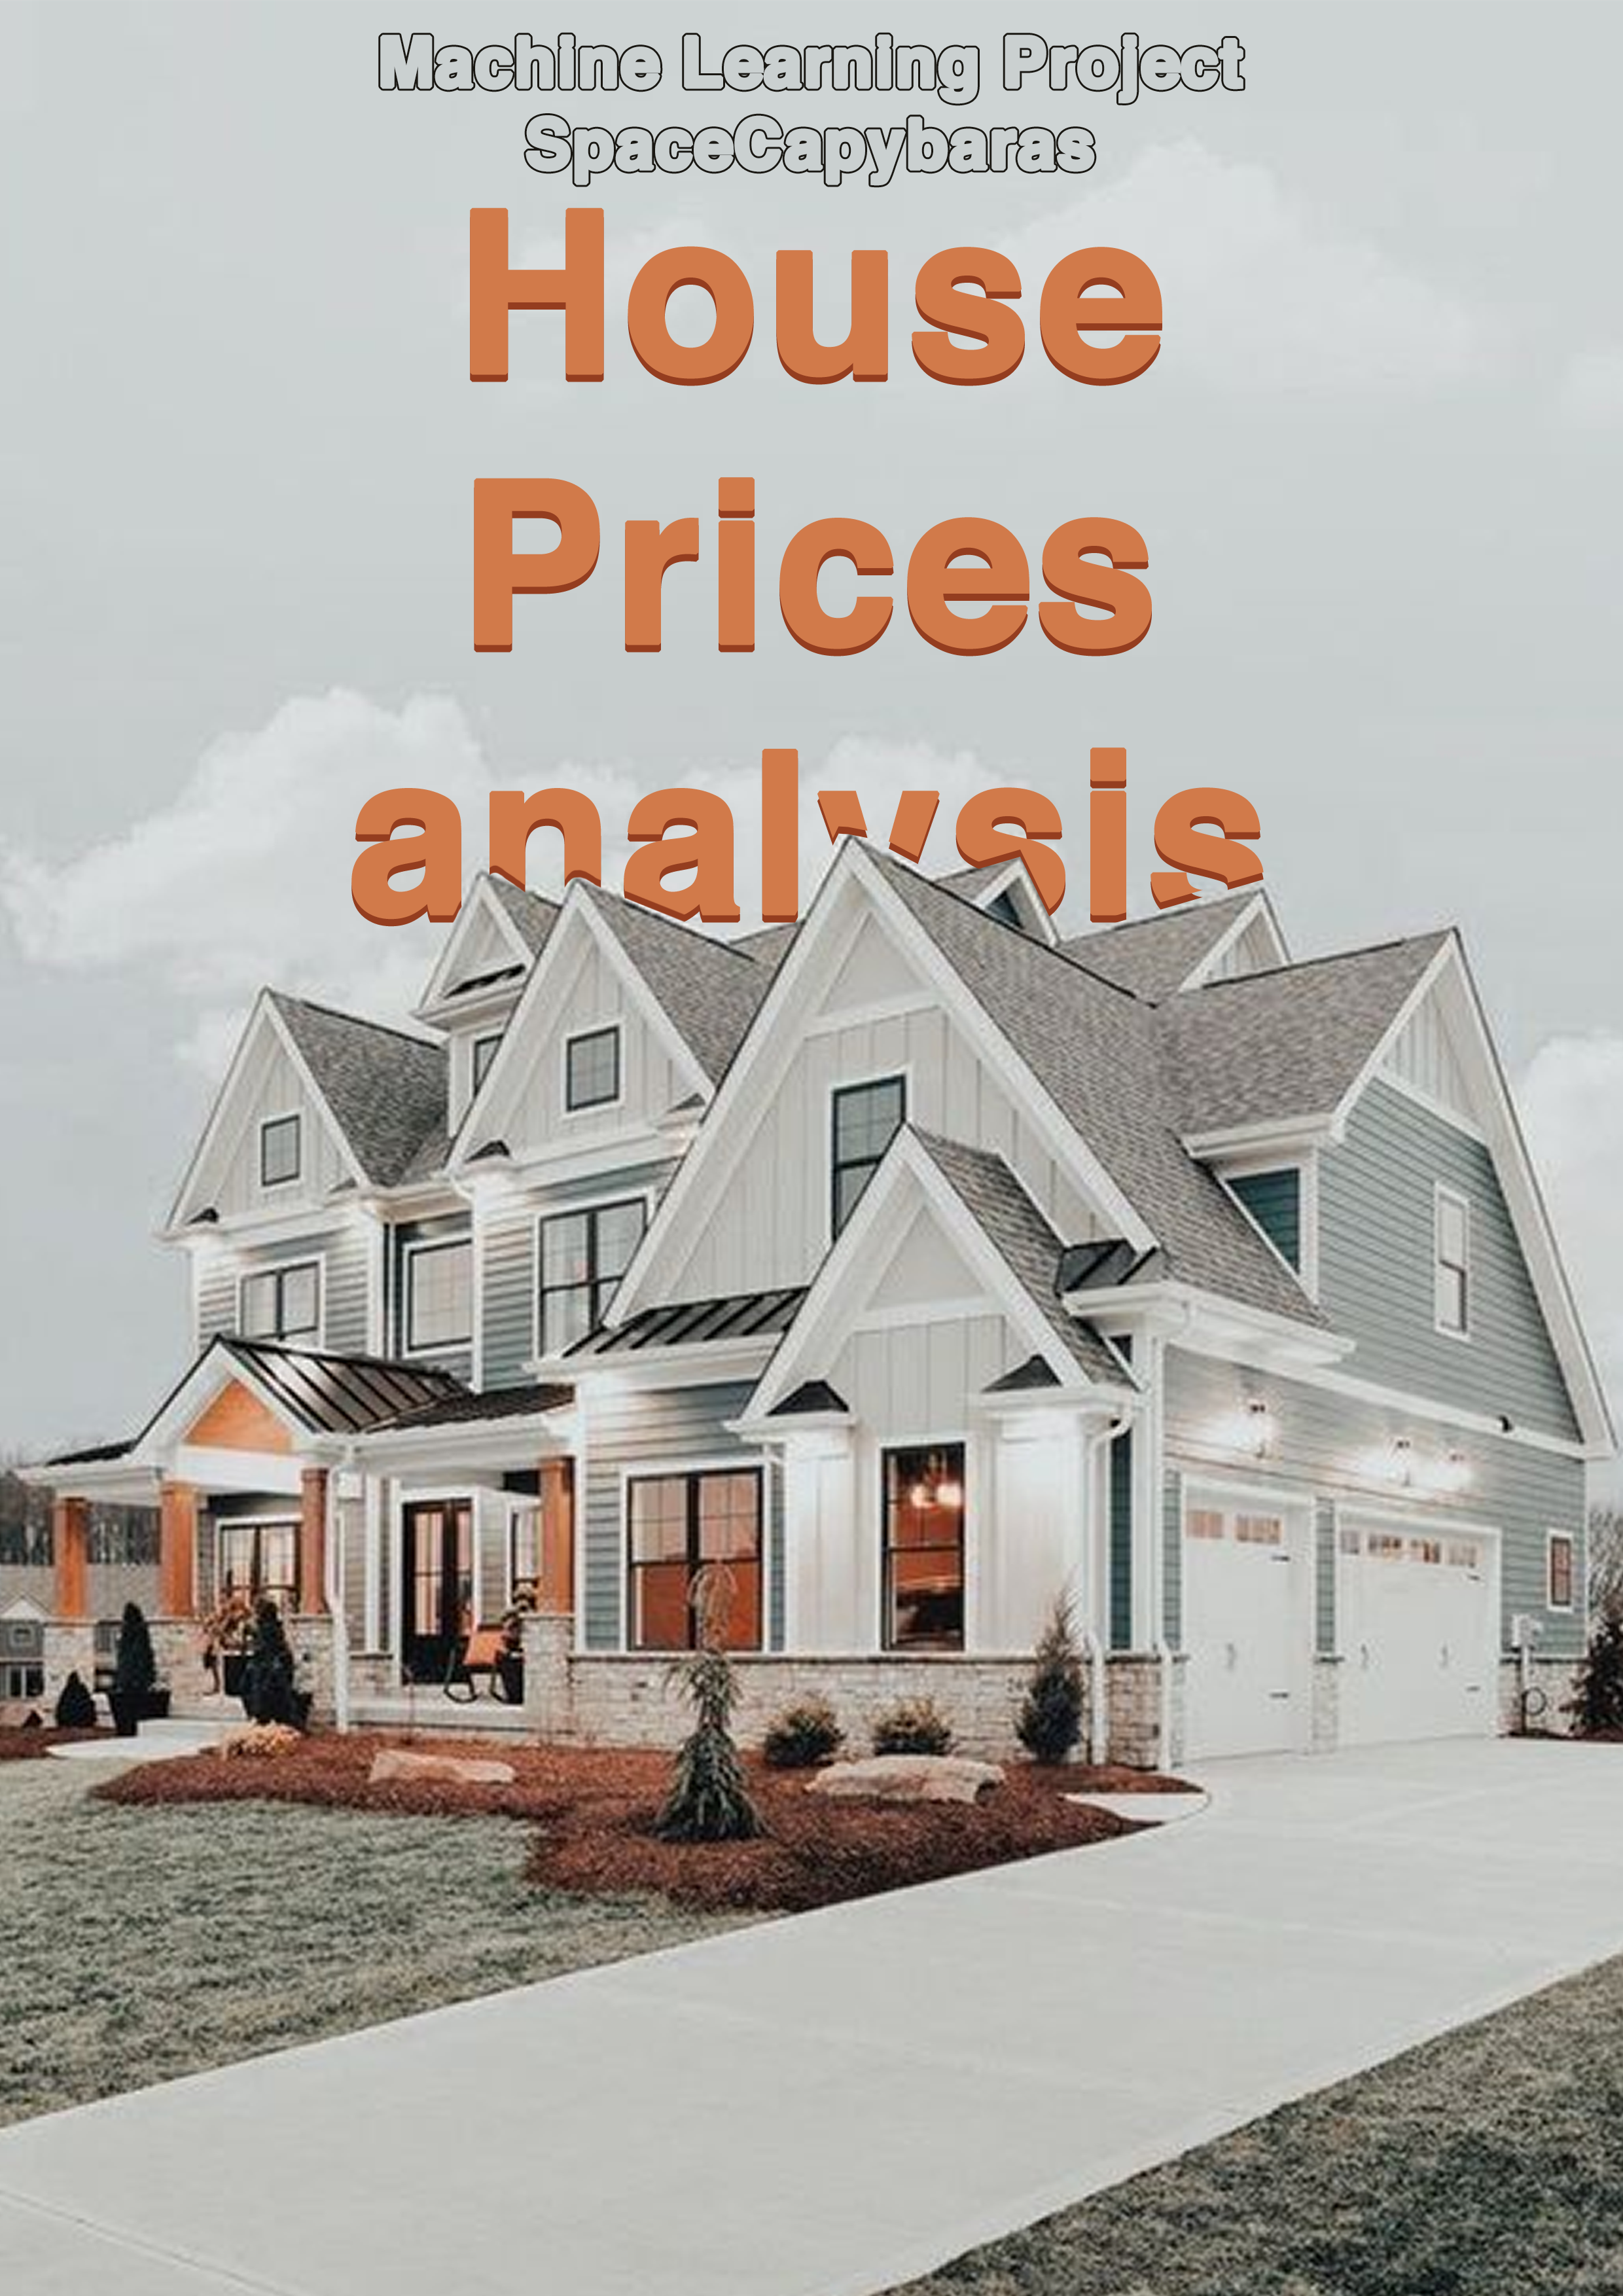
\includegraphics[width=\paperwidth,height=\paperheight]{imgs/project cover.png}
    }
\end{titlepage}

\tableofcontents



\newpage



\section{Introduction}
\label{sec:introduction}

To develop this \textbf{Machine Learning} project we are going to use the CRISP-DM methodology, which is a well-known and widely used methodology for data mining projects. It is an iterative process that is composed of six phases.

In particulal, the phases are:
\begin{enumerate}
    \item \textbf{Business Understanding}: in this phase we will try to understand the problem and the objectives of the project. We will also try to understand the data that we have at our disposal and how we can use it to solve the problem.
    \item \textbf{Data Understanding}: in this phase we will try to understand the data that we have at our disposal. We will try to understand the meaning of the data and how we can use it to solve the problem.
    \item \textbf{Data Preparation}: in this phase we will try to prepare the data for the next phases. We will try to clean the data and to transform it in a way that will be useful for the next phases.
    \item \textbf{Modeling}: in this phase we will try to build a model that will be able to solve the problem. We will try to find the best model for our problem.
    \item \textbf{Evaluation}: in this phase we will try to evaluate the model that we have built. We will try to understand if the model is good enough to solve the problem.
    \item \textbf{Deployment}: in this phase we will try to deploy the model that we have built. We will try to understand how we can use the model to solve the problem.
\end{enumerate}


\section{Business understanding}
\label{sec:business_understanding}

\subsection{Background}
Our project is based using the dataset of the Kaggle competition \href{https://www.kaggle.com/c/house-prices-advanced-regression-techniques}{House Prices: Advanced Regression Techniques}. 

The goal of the competition is to predict the final price of each home based on 79 explanatory variables describing (almost) every aspect of residential homes in Ames, Iowa.
The dataset is composed by 1460 rows and 81 columns, where the last column is the target variable, the Sale Price.

A small list of the variables is the following:

\begin{itemize}
    \item \textbf{LotArea}: Lot size in square feet
    \item \textbf{OverallQual}: Overall material and finish quality
    \item \textbf{OverallCond}: Overall condition rating
    \item \textbf{YearBuilt}: Original construction date
    \item \textbf{YearRemodAdd}: Remodel date
    \item \textbf{RoofStyle}: Type of roof
    \item \textbf{Exterior1st}: Exterior covering on house
    \item \textbf{Exterior2nd}: Exterior covering on house (if more than one material)
    \item \textbf{MasVnrType}: Masonry veneer type
    \item \textbf{MasVnrArea}: Masonry veneer area in square feet
    \item \dots
\end{itemize}
\subsection{Business objectives}
\label{subsec:business_objectives}

In this part we are going to analyze the business objective of the project.
Our goal is different from the one of the competition, in fact we are requested to \textbf{convert the Sale Price variable into 3 ranges}:

\begin{enumerate}
    \item \textbf{LOW}: From 0 to 150000 
    \item \textbf{MEDIUM}: From 150000 to 300000 
    \item \textbf{HIGH}: From 300000 and beyond 
\end{enumerate}

The dataset 




\chapter{Data understanding}
\label{sec:data_understanding}

\section{Data description}
\label{sec:data_description}

The dataset we are using, House Prices - Advanced Regression Techniques, is a dataset containing 79 explanatory variables describing (almost) every aspect of residential homes in Ames, Iowa. The dataset is composed of 1460 rows, each one representing a house, and 81 columns, 80 of which are features and 1 is the target variable, the SalePrice.

With the dataset is provided a \textit{data description} with the description for each variable in thedataset.

%split the table in two parts
\begin{table}[H]
    \centering
    \begin{longtable}{|l|l|}
        \hline
        Variable      & Description                                                 \\
        \hline
        SalePrice     & The property's sale price in dollars. (Target variable)     \\
        \hline
        MSSubClass    & The building class                                          \\
        \hline
        MSZoning      & The general zoning classification                           \\
        \hline
        LotFrontage   & Linear feet of street connected to property                 \\
        \hline
        LotArea       & Lot size in square feet                                     \\
        \hline
        Street        & Type of road access                                         \\
        \hline
        Alley         & Type of alley access                                        \\
        \hline
        LotShape      & General shape of property                                   \\
        \hline
        LandContour   & Flatness of the property                                    \\
        \hline
        Utilities     & Type of utilities available                                 \\
        \hline
        LotConfig     & Lot configuration                                           \\
        \hline
        LandSlope     & Slope of property                                           \\
        \hline
        Neighborhood  & Physical locations within Ames city limits                  \\
        \hline
        Condition1    & Proximity to main road or railroad                          \\
        \hline
        Condition2    & Proximity to main road or railroad (if a second is present) \\
        \hline
        BldgType      & Type of dwelling                                            \\
        \hline
        HouseStyle    & Style of dwelling                                           \\
        \hline
        OverallQual   & Overall material and finish quality                         \\
        \hline
        OverallCond   & Overall condition rating                                    \\
        \hline
        YearBuilt     & Original construction date                                  \\
        \hline
        YearRemodAdd  & Remodel date                                                \\
        \hline
        RoofStyle     & Type of roof                                                \\
        \hline
        RoofMatl      & Roof material                                               \\
        \hline
        Exterior1st   & Exterior covering on house                                  \\
        \hline
        Exterior2nd   & Exterior covering on house (if more than one material)      \\
        \hline
        MasVnrType    & Masonry veneer type                                         \\
        \hline
        MasVnrArea    & Masonry veneer area in square feet                          \\
        \hline
        ExterQual     & Exterior material quality                                   \\
        \hline
        ExterCond     & Present condition of the material on the exterior           \\
        \hline
        Foundation    & Type of foundation                                          \\
        \hline
        BsmtQual      & Height of the basement                                      \\
        \hline
        BsmtCond      & General condition of the basement                           \\
        \hline
        BsmtExposure  & Walkout or garden level basement walls                      \\
        \hline
        BsmtFinType1  & Quality of basement finished area                           \\
        \hline
        BsmtFinSF1    & Type 1 finished square feet                                 \\
        \hline
        BsmtFinType2  & Quality of second finished area (if present)                \\
        \hline
        BsmtFinSF2    & Type 2 finished square feet                                 \\
        \hline
        BsmtUnfSF     & Unfinished square feet of basement area                     \\
        \hline
        TotalBsmtSF   & Total square feet of basement area                          \\
        \hline
        Heating       & Type of heating                                             \\
        \hline
        HeatingQC     & Heating quality and condition                               \\
        \hline
        CentralAir    & Central air conditioning                                    \\
        \hline
        Electrical    & Electrical system                                           \\
        \hline
        1stFlrSF      & First Floor square feet                                     \\
        \hline
        2ndFlrSF      & Second floor square feet                                    \\
        \hline
        LowQualFinSF  & Low quality finished square feet (all floors)               \\
        \hline
        GrLivArea     & Above grade (ground) living area square feet                \\
        \hline
        BsmtFullBath  & Basement full bathrooms                                     \\
        \hline
        BsmtHalfBath  & Basement half bathrooms                                     \\
        \hline
        FullBath      & Full bathrooms above grade                                  \\
        \hline
        HalfBath      & Half baths above grade                                      \\
        \hline
        Bedroom       & Number of bedrooms above basement level                     \\
        \hline
        Kitchen       & Number of kitchens                                          \\
        \hline
        KitchenQual   & Kitchen quality                                             \\
        \hline
        TotRmsAbvGrd  & Total rooms above grade (does not include bathrooms)        \\
        \hline
        Functional    & Home functionality rating                                   \\
        \hline
        Fireplaces    & Number of fireplaces                                        \\
        \hline
        FireplaceQu   & Fireplace quality                                           \\
        \hline
        GarageType    & Garage location                                             \\
        \hline
        GarageYrBlt   & Year garage was built                                       \\
        \hline
        GarageFinish  & Interior finish of the garage                               \\
        \hline
        GarageCars    & Size of garage in car capacity                              \\
        \hline
        GarageArea    & Size of garage in square feet                               \\
        \hline
        GarageQual    & Garage quality                                              \\
        \hline
        GarageCond    & Garage condition                                            \\
        \hline
        PavedDrive    & Paved driveway                                              \\
        \hline
        WoodDeckSF    & Wood deck area in square feet                               \\
        \hline
        OpenPorchSF   & Open porch area in square feet                              \\
        \hline
        EnclosedPorch & Enclosed porch area in square feet                          \\
        \hline
        3SsnPorch     & Three season porch area in square feet                      \\
        \hline
        ScreenPorch   & Screen porch area in square feet                            \\
        \hline
        PoolArea      & Pool area in square feet                                    \\
        \hline
        Pool Area     & Pool area in square feet                                    \\
        \hline
        PoolQC        & Pool quality                                                \\
        \hline
        Fence         & Fence quality                                               \\
        \hline
        MiscFeature   & Miscellaneous feature not covered in other categories       \\
        \hline
        MiscVal       & Value of miscellaneous feature in dollars                   \\
        \hline
        MoSold        & Month Sold                                                  \\
        \hline
        YrSold        & Year Sold                                                   \\
        \hline
        SaleType      & Type of sale                                                \\
        \hline
        SaleCondition & Condition of sale                                           \\
        \hline
    \end{longtable}

    \caption{Data description (1/2)}
    \label{tab:data_description_1}

\end{table}

\end{document}
